  \section{Examples}
\label{sec:examples}
  In this section, the efficacy of the proposed method is evaluated through the two examples introduced in Sec.\ref{sec:preliminaries}. The relaxed problems were parsed using the SPOTLESS toolbox \cite{spotless} and were numerically solved with MOSEK on a computer equipped with a Intel Xeon W3540 processor and 12GB of RAM.
  The following points on the examples considered are obligatory.
  \begin{enumerate}
    \item It is a characteristic trait of the problem formulation considered in this paper that the actual distribution of the uncertainty is immaterial. Consequently, in all examples, it is assumed that the disturbance, $\theta$, is uniformly distributed. For notional convenience, $\theta\sim\mathcal U([a,b])$ is used to denote that $\theta$ is uniformly distributed in the interval $[a,b]$.
    \item For reasons related to numerics, all problems are normalized such that the state-space is given by $[-1,1]^n$, for an appropriate value of $n$.
  \end{enumerate}
  Also, since has been established that the solution of relaxed problems provides an outer approximation of the BRS, in this section, the qualifier `approximate' is suppressed.
  \subsection{1-D linear dynamics}
  As a review, we consider a (non-hybrid) 1-D linear dynamical system whose dynamics is given by
  \begin{align}
	\dot x_1 = -0.7x_1+0.2\theta-0.1,
\end{align}
where $\theta\in \mathcal U([0.2,1])$.
Although this system is hybridizable as discussed in Ex.~\ref{example:1D}, in the version considered here, we do not hybridize its dynamics. The target set to which trajectories must reach in one second is set as $X_T=[0.2,0.4]$. The BRS of the deterministic system which assumes that $\theta$ is a known constant is analytically computed to equal

\tiny
\begin{align*}
  BRS_\theta=\left[\left(0.2-\frac{2\theta-1}{7}\right)e^{0.7}-\frac{2\theta-1}{7}, \left(0.4-\frac{2\theta-1}{7}\right)e^{0.7}-\frac{2\theta-1}{7}\right]
\end{align*}
\normalsize
Note that the expression for the $BRS_\theta$ is linear in $\theta$ and that the width of $BRS_\theta$ is constant for all values of $\theta$. As the value of $\theta$ changes, $BRS_\theta$ slides along $\R$; the intersection of $BRS_0$ and $BRS_1$ is the BRS of the uncertain system, as defined in Eqn.~(\ref{eq:brs}).
\par
Figure~\ref{fig:1D:linear} presents the degree 12 approximation of the indicator function that is supported on the BRS of the uncertain system, $w^{12}$, for cases when $\theta$ takes a constant value and when it is drawn at random. The graphs in green and cyan correspond to the cases when $\theta$ takes a constant value of $\theta=0$ and $\theta=1$ respectively. The red trace is the polynomial solution to the uncertain problem. Observe that the BRS corresponding to uncertain case encloses the intersection of those of the deterministic of cases; this is the desired outcome.
\begin{figure}[!t]
  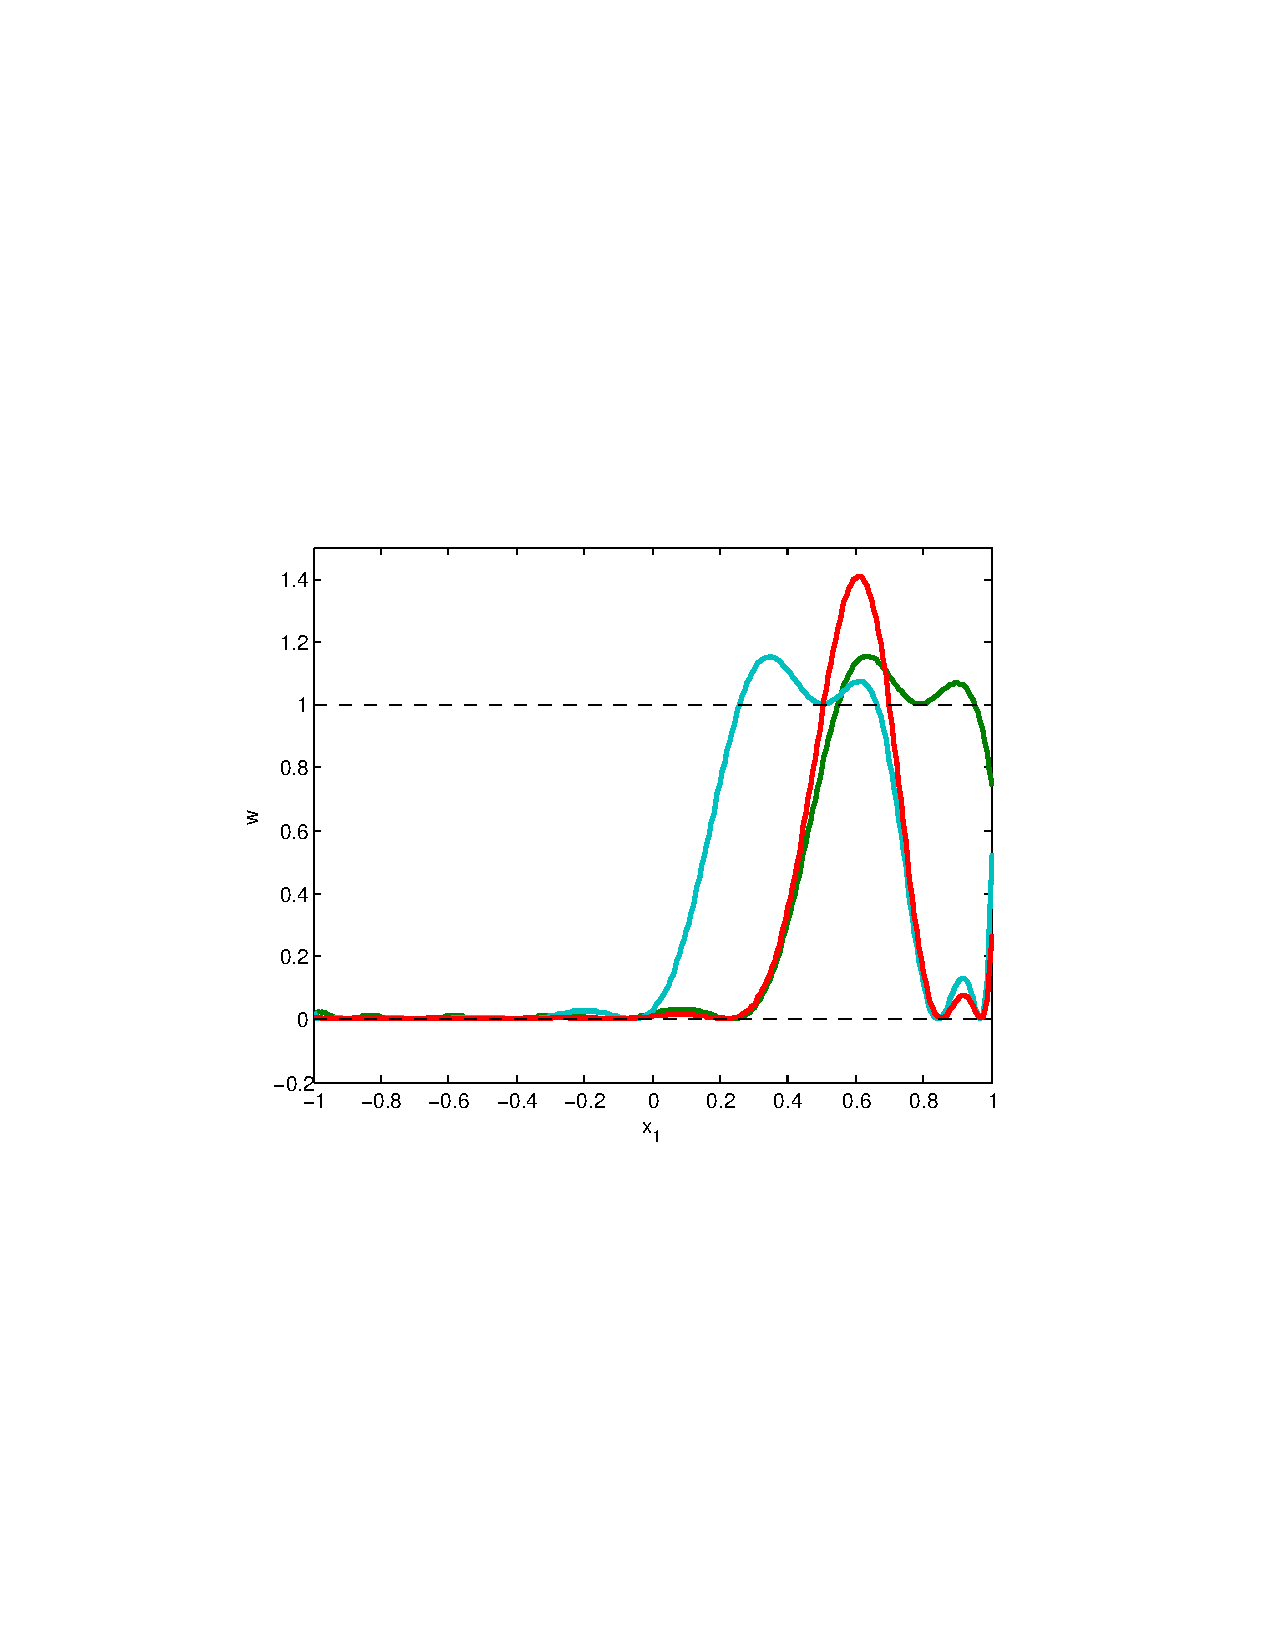
\includegraphics[width=\columnwidth,trim =1.5in 3.3in 1.5in 3.5in, clip=true]{figures/1D_3}
  \caption{Outer approximations of the BRS of the extreme deterministic cases and the stochastic case.(green) $\theta=0$, (blue) $\theta=1$ and (red) $\mu_\theta$}
    \label{fig:1D:linear}
\end{figure}
\subsection{Planar rimless wheel (PRW)}
The rolling PRW, introduced in Ex.\ref{example:rw}, is a one mode hybrid system in which the guard is reached when the marching foot makes contact with the wedge. For a PRW rolling along a {\em smooth} wedge, an analytically computable stable limit cycle exits \cite{Coleman1998}; however, for the case considered in this example---with the wedge face having undulations---the definition of a limit cycle less clear. Consequently, a notion of {\em meta-stability}---when the system states arrive within $\epsilon$ of the stable limit cycle of the disturbance-free system---is adopted.
\par
Figure~\ref{fig:rw_brs} presents the polynomial degree 12 BRS (black dashed) for the rimless wheel (with $\alpha=0.4$) which is tasked with arriving within the red band in $T=4$ seconds, as it is rolling down a wedge with slope $\gamma=0.2$ withstanding an a sequence of random changes to terrain drawn from $\theta\sim\mathcal U([-0.1,0.1])$. The relative depths/height of the disturbance is about 25\% the length of each spoke.
\par
The BRS is validated by performing Monte Carlo simulations; the box $I^2$ is discretized into 51 points both ways and 100 independent trajectories are simulated (using MATLAB's {\em ode45} function) from each initial condition. The blue $\cdot$s depict the initial conditions that arrived within the terminal set at the desired time without violating any of the other constraints. Note that the set of points that succeeded in the MC simulation is entirely contained in the BRS.
\begin{figure}[!t]
  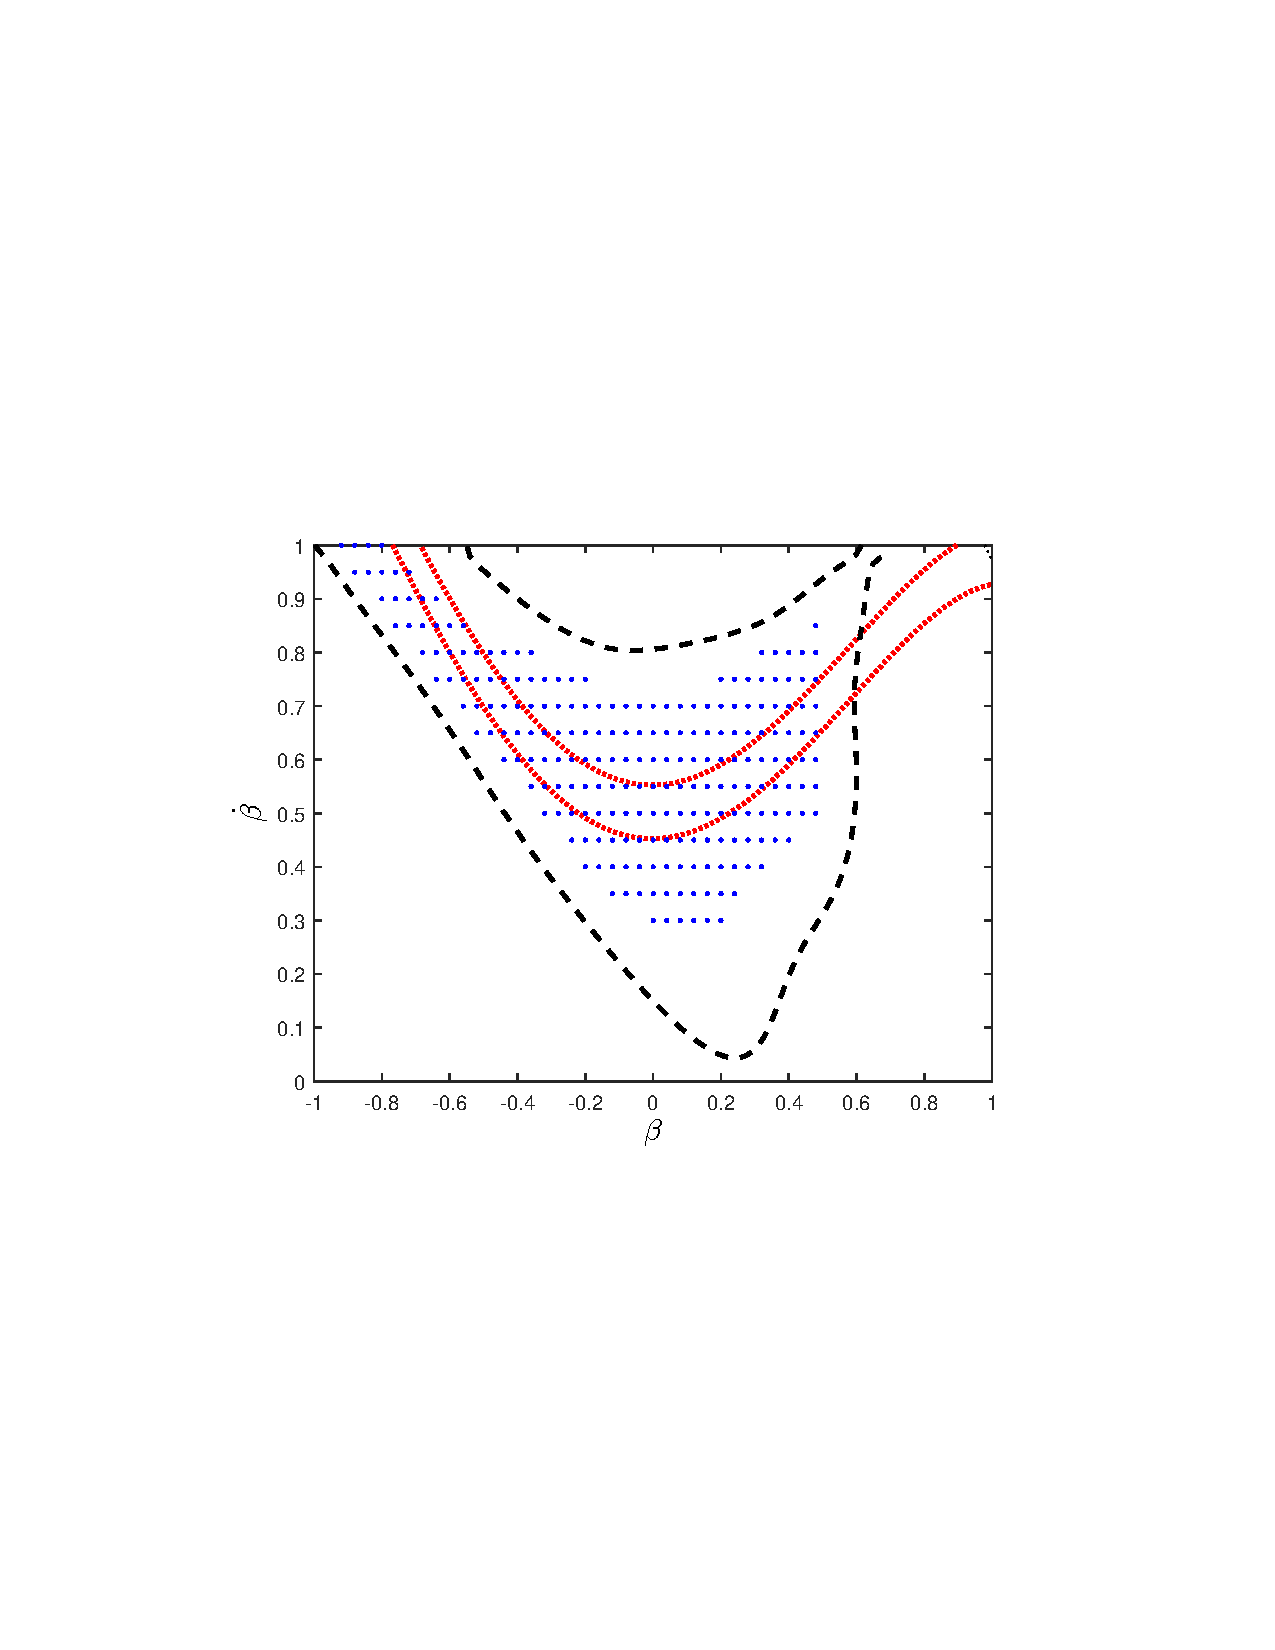
\includegraphics[trim=1.5in 3.3in 1.5in 3.5in, clip=true,width=\columnwidth]{figures/rw_0p1_4_new}
  \caption{Outer approximation and estimated BRS based on 100 iterations and T=4. Red band is the terminal set and the black outer is the boundary of the estimated BRS; the crosses correspond to results of MC simulation.}
  \label{fig:rw_brs}
\end{figure}
\par
At this juncture, a remark about the tightness of the BRS is warranted. Clearly, the BRS in Fig.~\ref{fig:rw_brs} is not tight; and we attribute this to the set of basis functions with which are currently working--monomials; and the degree relaxation. As commented in \cite{henrion2014convex}, adopting an alternate basis set is likely to increase the rate of convergence and the tightness. As it stands, there are alternate ways to improve the tightness, primary amongst which is to create phantom modes using identity reset maps; this approach however, needs some care and is deferred for a future work.
